\subsection{The Six Bar Cosmic-Ray Method}
The six bar method cosmic-ray method (hereafter known as the six bar
method) consists of six simultaneous three bar measurements.  The
system of equations for the counter resolutions that arises due to
Gaussian error propagation is then solved for the individual counter
resolutions.

Analogous to the three counters in the three bar method, six
identical-length counters are stacked vertically and equally-spaced,
and events are selected according to the requirement that the
cosmic-ray particle was detected by all six counters.  Labeling the
counters 1 through 6, starting with the top counter, and using the
notation (top, middle, bottom) to represent the counters involved in
each three bar measurement, the three-bar measurements performed are:
(1,2,3), (2,3,4), (3,4,5), (4,5,6), (1,3,5), and (2,4,6).  These are
the only possible combinations of three counters in which the spacing
between adjacent counters is the same.

\begin{figure}[H]
  \centering
  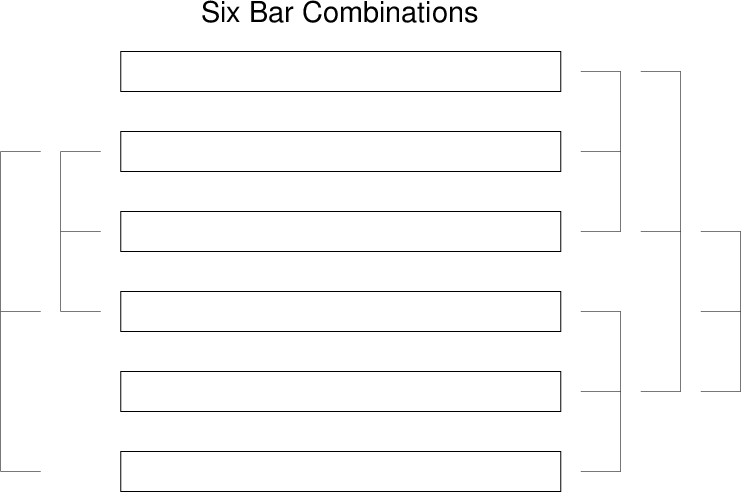
\includegraphics[width=15cm]{gary/fig_gary_six_bar_method/6bar.png}
  \caption{Depiction of which three bar combinations are selected for
    the six bar method.}
  \label{6bar}
\end{figure}

Using $t_n$ for the cosmic-ray interaction times through the
$n\mathrm{th}$ counter, the three-bar method observables for each of
the six combinations of three counters are given by:

\[T_{(1,2,3)} = (t_1 + t_3)/2 - t_2,\]
\[T_{(2,3,4)} = (t_2 + t_4)/2 - t_3,\]
\[T_{(3,4,5)} = (t_3 + t_5)/2 - t_4,\]
\[T_{(4,5,6)} = (t_4 + t_6)/2 - t_5,\]
\[T_{(1,3,5)} = (t_1 + t_5)/2 - t_3,\]
\[T_{(2,4,6)} = (t_2 + t_6)/2 - t_4.\]

Applying error propagation to the above equations, this system of
equations for the counter resolutions follows:

\[\begin{cases}
\sigma_{T_{(1,2,3)}}^2 = (\sigma_1^2 + \sigma_3^2)/4 + \sigma_2^2\\
\sigma_{T_{(2,3,4)}}^2 = (\sigma_2^2 + \sigma_4^2)/4 + \sigma_3^2\\
\sigma_{T_{(3,4,5)}}^2 = (\sigma_3^2 + \sigma_5^2)/4 + \sigma_4^2\\
\sigma_{T_{(4,5,6)}}^2 = (\sigma_4^2 + \sigma_6^2)/4 + \sigma_5^2\\
\sigma_{T_{(1,3,5)}}^2 = (\sigma_1^2 + \sigma_5^2)/4 + \sigma_3^2\\
\sigma_{T_{(2,4,6)}}^2 = (\sigma_2^2 + \sigma_6^2)/4 + \sigma_4^2
\end{cases}\]

Written in matrix form, the system of equations is:

\[\left[\begin{array}{c}
    \sigma_{T_{(1,2,3)}}^2 \\
    \sigma_{T_{(2,3,4)}}^2 \\
    \sigma_{T_{(3,4,5)}}^2 \\
    \sigma_{T_{(4,5,6)}}^2 \\
    \sigma_{T_{(1,3,5)}}^2 \\
    \sigma_{T_{(2,4,6)}}^2 \\
  \end{array}
  \right]
= \left[ \begin{array}{cccccc}
    \frac{1}{4} & 1 & \frac{1}{4} & 0 & 0 & 0 \\
    0 & \frac{1}{4} & 1 & \frac{1}{4} & 0 & 0 \\
    0 & 0 & \frac{1}{4} & 1 & \frac{1}{4} & 0 \\
    0 & 0 & 0 & \frac{1}{4} & 1 & \frac{1}{4} \\
    \frac{1}{4} & 0 & 1 & 0 & \frac{1}{4} & 0 \\
    0 & \frac{1}{4} & 0 & 1 & 0 & \frac{1}{4}\\
  \end{array}
  \right]
\left[
  \begin{array}{c}
    \sigma_1^2 \\
    \sigma_2^2 \\
    \sigma_3^2 \\
    \sigma_4^2 \\
    \sigma_5^2 \\
    \sigma_6^2 \\
  \end{array}
  \right]\]

Since the determinant of the coefficient matrix is non-zero
($81/1024$), the system is independent and can be solved to yield the
\(\sigma_i^2\) by one of the many available techniques to solve a
linear system of equations.
